\documentclass[]{article}
\usepackage[a4paper, total={15cm,23cm}]{geometry}
\usepackage{fancyhdr}
\usepackage{graphicx}
\usepackage{amsmath}
\usepackage{amssymb}
\usepackage{xcolor}
\usepackage{tikz}
%opening
\title{PH 223 Week 1}
\author{Benjamin Bauml, Danielle Skinner, Grant Sherer}
\date{Winter 2024}
\pagestyle{fancy}
\rhead{PH 223}
\chead{Winter 2024}
\lhead{Week 1}

%Custom Quotation Command
\newcommand{\excerpt}[1]{\colorbox{lightgray}{\parbox{14.8cm}{#1}} \\}

\begin{document}

\maketitle

\begin{center}
Activity 1 is borrowed/adapted from Chapter 22 of \textit{Physics for Scientists and Engineers}.
\end{center}
\section*{Activity 1}
\excerpt{
What mass of aluminum has a total nuclear charge of 1.0 C? Aluminum has atomic number 13 and molar mass 26.98 g/mol.
}
Let $ N $ be the number of aluminum atoms, and let $ m $ be the mass we are looking for. It follows that the total charge $ Q = 13eN $ (where $ e = 1.60\times10^{-19} $ C is the charge on a single proton). We know that there are approximately $ 6.022\times10^{23} $ aluminum atoms in one mole of aluminum, and each mole has 0.02698 kg of mass. By using these ratios to convert units, we find
\[
\begin{split}
	m & = N \frac{1\text{ mol Al}}{6.022\times10^{23}\text{ Al atoms}} \frac{0.02698\text{ kg}}{1\text{ mo Al}} \\
	& = \frac{Q}{13e} \frac{0.02698\text{ kg}}{6.022\times10^{23}} \\
	& = \frac{1.0\text{ C}}{13(1.60\times10^{-19}\text{ C})} \frac{0.02698\text{ kg}}{6.022\times10^{23}} \\
	& \approx 2.15\times10^{-8}\text{ kg}.
\end{split}
\]
The mass of aluminum with the desired nuclear charge is 21.5 nkg, which is minuscule; this illustrates how small atoms and protons are. Due to the equal number of electrons present, this chunk of aluminum would likely be close to neutral.

\section*{Activity 2}
\excerpt{
You dip a candy bar into chocolate and pull it out slowly so that more and more chocolate accu- mulates on the bar. When the chocolate has cooled, you measure the mass density at one end to be $\lambda = 0$ and the density at the other end to be $\lambda = \alpha L$, where $L$ is the length of the bar and $\alpha$ is a constant, and you assume the mass density is linearly proportional to distance along the candy bar.
}
\excerpt{
(a) How are $\lambda$, mass, and length related?
}
Here, $\lambda$ is the linear mass density, which has dimensions of mass divided by length (and thus, commonly it has units of kg/m). In a given material, it tells us how mass is concentrated along a given direction. Taking a segment of the material characterized by some length along that direction, the density allows us to figure out how much mass is in that segment. \\
\excerpt{
(b) Can you represent this relationship as a derivative?
}
Linear mass density can be represented as a derivative of mass with respect to position:
\[
\lambda = \frac{dm}{dx}.
\]
Rearranging this into the form $dm = \lambda dx$ gives us the intuitive picture that multiplying an infinitesimal bit of length by the linear density gives us the infinitesimal bit of mass in that region. This corresponds to our common understanding that a uniform linear mass density multiplied by the total length of the material gives the material's total mass. The derivative form here is more general. \\
\excerpt{
(c) Determine the total mass of chocolate on the candy bar.
}
When mass density varies, we cannot just multiply the density by the length. Instead, we add up every infinitesimal piece of mass through integration to get the total mass:
\[
M_{total} = \int dm.
\]
Rather than integrate mass directly, we use $dm = \lambda dx$ to instead integrate with respect to length. Integrating from one end of the chocolate bar to the other gives us the bounds $0$ and $L$:
\[
M_{total} = \int_{0}^{L}\lambda dx.
\]
Now, what is $\lambda$? By ``linearly proportional,'' we mean that $\lambda$ is an equation which is linear with respect to the variable $x$, and we know that we start with $\lambda = 0$ at $x = 0$ and end with $\lambda = \alpha L$ at $x = L$. This is accomplished by
\[
\lambda(x) = \alpha x.
\]
Substituting this into our integral, we get
\[
M_{total} = \int_{0}^{L}\alpha x dx = \alpha \left[\frac{1}{2}x^{2}\right]_{x=0}^{L} = \frac{1}{2}\alpha L^{2}.
\]
Note that $\alpha$ must have dimensions of mass divided by area, perhaps requiring units of kg/m$^{2}$. For something the size of a candy bar, g/cm$^{2}$ might be a more appropriate choice, but either works. \\
\excerpt{
(d) The expression for center of mass is 
\begin{equation}
	x_{cm} = \frac{1}{m_i}\int_{x_i}^{x_f} x dm
\end{equation}
Use this expression to find the center of mass of the chocolate bar.
}
The center of mass integral averages each point along the object, weighted by the mass at that point. Again, rather than integrate with respect to mass, we rewrite the mass in terms of the position, obtaining
\[
x_{cm} = \frac{1}{M_{total}}\int_{0}^{L} x \lambda(x) dx = \frac{1}{M_{total}}\int_{0}^{L} \alpha x^{2} dx = \frac{\alpha L^{3}}{3M_{total}} = \frac{2}{3}L.
\]
As we might expect, the center of mass is closer to the end of the chocolate bar which has a higher density.

\section*{Activity 3}
\excerpt{
For each of the following charge density distributions, determine the units of the constant of proportionality ($\alpha, \beta, \gamma$) and the total charge.
}
For (a) and (b), we are dealing with linear charge density $\lambda$, which should have dimensions of charge (which I symbolize as Q) divided by length (which I shall symbolize as L). Notationally, I indicate that $\lambda$ has these dimensions with the expression
\[
[\lambda] = \frac{\text{Q}}{\text{L}}.
\]
Analogously, a linear mass density could be said to have dimension $\frac{\text{M}}{\text{L}}$, with M being the dimension of mass.

For (c), we are dealing with surface charge density $\sigma$, which should have dimensions of charge divided by area (or length squared), which I indicate with the expression
\[
[\sigma] = \frac{\text{Q}}{\text{L}^{2}}.
\]

Using dimensions in this way is a powerful tool that serves the same role as a unit check without being linked to a particular system of units. The following solution will work with dimensions, but if you wish to work with SI base units, you could replace Q with C for coulombs and L with m for meters.

Unfortunately, this convention I am using may be confusing, as I will be using Q and L in two slightly different ways. For dimensions, I will use unitalicized characters, whereas symbolic constants and variables will use italicized characters. In particular, Q is the dimension of charge, $Q$ is the net charge of an object (which is what we will be solving for), L is the dimension of length, and $L$ is the length of the rods in parts (a) and (b). \\
\excerpt{
(a) A rod of length $L$ oriented along the x-axis with charge distribution $\lambda (x) = \alpha x^{1/3}$.
}
We know that $[\lambda] = \frac{\text{Q}}{\text{L}}$, and $x$ is a position, so $[x]=\text{L}$. It must be true that
\[
\begin{split}
	\left[\alpha x^{1/3}\right] & = [\lambda] \\
	[\alpha] [x]^{1/3} & = [\lambda] \\
	[\alpha] \text{L}^{1/3} & = \frac{\text{Q}}{\text{L}} \\
	[\alpha] & = \frac{\text{Q}}{\text{L}^{4/3}}.
\end{split}
\]
Thus, $\alpha$ has dimensions of charge divided by length taken to the power of $\frac{4}{3}$.

Getting the total charge is just like getting total mass from a linear mass density. In this case, $\lambda = \frac{dq}{dx}$, and the total charge $Q$ is
\[
Q = \int dq = \int_{0}^{L}\lambda(x)dx = \int_{0}^{L} \alpha x^{1/3} dx = \alpha\left[\frac{3}{4}x^{4/3}\right]_{x=0}^{L} = \frac{3}{4}\alpha L^{4/3}.
\]
Note that the dimensions of $\alpha$ cancel partially with the dimensions of $L^{4/3}$ to leave only charge, so the dimensions of this expression are correct. \\
\excerpt{
(b) A rod of length $L$ oriented along the y-axis with charge distribution $\lambda (y) = \beta y^{5}$.
}
For the dimensions of $\beta$, we find that
\[
\begin{split}
	\left[\beta y^{5}\right] & = [\lambda] \\
	[\beta] [y]^{5} & = [\lambda] \\
	[\beta] \text{L}^{5} & = \frac{\text{Q}}{\text{L}} \\
	[\beta] & = \frac{\text{Q}}{\text{L}^{6}}.
\end{split}
\]
The total charge is
\[
Q = \int dq = \int_{0}^{L}\lambda(y)dy = \int_{0}^{L} \beta y^{5} dy = \beta\left[\frac{1}{6}y^{6}\right]_{y=0}^{L} = \frac{1}{6}\beta L^{6}.
\]
\newpage
\noindent\excerpt{
(c) A disk of radius $R$ with charge distribution $\sigma (x,y) = \gamma xy$.
}
For the dimensions of $\gamma$, we find that
\[
\begin{split}
	\left[\gamma xy\right] & = [\sigma] \\
	[\gamma] [x][y] & = [\sigma] \\
	[\gamma] \text{L}^{2} & = \frac{\text{Q}}{\text{L}^{2}} \\
	[\gamma] & = \frac{\text{Q}}{\text{L}^{4}}.
\end{split}
\]
Since we are working with a cylindrically symmetric object, let us use polar coordinates. That means we will be using the relationships $x=r\cos\theta$ and $y=r\sin\theta$, and the area element will be $dA=rdrd\theta$. Here, $\sigma = \frac{dq}{dA}$, so $dq = \sigma rdrd\theta$. The total charge is
\[
\begin{split}
	Q = \int dq & = \int_{0}^{2\pi}\int_{0}^{R}\sigma(x,y)rdrd\theta \\
	& = \int_{0}^{2\pi}\int_{0}^{R}\gamma xyrdrd\theta \\
	& = \gamma \int_{0}^{2\pi}\int_{0}^{R}(r\cos\theta)(r\sin\theta)rdrd\theta \\
	& = \gamma \int_{0}^{2\pi}\cos\theta\sin\theta d\theta \int_{0}^{R}r^{3}dr.
\end{split}
\]
At this point, note that
\[
\int_{0}^{2\pi}\cos\theta\sin\theta d\theta = \left[\frac{1}{2}\sin^{2}\theta\right]_{\theta=0}^{2\pi} = 0,
\]
so the disk has zero net charge ($Q = 0$ C)! This does not mean it is completely neutral at all points---it has an equal amount of positive and negative charge overall, but that charge is distributed unevenly (with net positive charge in two opposite quarters and net negative charge in the other two quarters; the image below depicts this arrangement, assuming $\gamma$ is positive).
\begin{center}
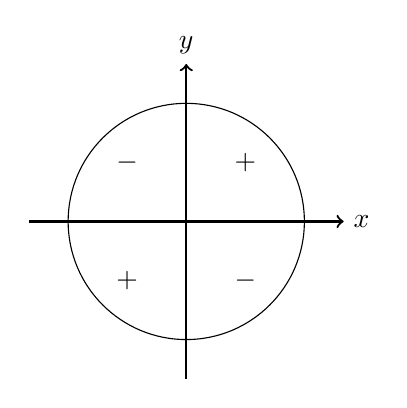
\begin{tikzpicture}
	\draw[->,thick] (-2,0) -- (2,0);
	\node[anchor = west] at (2,0) {$x$};
	\draw[->,thick] (0,-2) -- (0,2);
	\node[anchor = south] at (0,2) {$y$};
	\draw (0,0) circle (1.5);
	\node at (0.75,0.75) {$+$};
	\node at (-0.75,0.75) {$-$};
	\node at (0.75,-0.75) {$-$};
	\node at (-0.75,-0.75) {$+$};
\end{tikzpicture}
\end{center}

\end{document}
